\documentclass[12pt]{article}
\usepackage[margin=1in]{geometry}
\usepackage{amsmath}
\usepackage{amssymb}
\usepackage{amsfonts}
\usepackage{amsthm}
\newtheorem{thm}{Theorem}[section]
\newtheorem{cor}[thm]{Corollary}
\newtheorem{lem}[thm]{Lemma}
\usepackage{tikz-cd}
\renewcommand{\d}{\mathrm{d}}

\begin{document}

\title{Math 180 Homework 3}
\author{Nathan Solomon}
\maketitle

\section{}
\noindent\fbox{\fbox{\parbox{6.5in}{
    Prove or disprove: if $u$ and $v$ are the only vertices in a graph with odd degree, then there is a path from $u$ to $v$.
}}}\bigskip\par
Assume this question is talking about simple graph, and not multigraphs. If multigraphs are allowed, there is an obvious counterexample: the graph with two vertices which each have one edge to themselves, but are not connected to each other.
\par
Suppose there exists a (simple) graph $G$ in which $u$ and $v$ are the only vertices with odd degree, and there is no path from $u$ to $v$. Then let $U$ be the connected component of $G$ which contains $u$ but not $v$. The only vertex in $U$ with odd degree is $u$, so the sum of the degrees of each vertex in $U$ is odd. But because $U$ is a simple graph, it must follow the handshaking lemma, so this is a contradiction. Therefore there must be a path in $G$ from $u$ to $v$.

\section{}
\noindent\fbox{\fbox{\parbox{6.5in}{
            Let $G$ be the complete bipartite graph $K_{m,n}$, where $m,n > 0$. Characterize the $m,n$ such that:
            \begin{itemize}
                \item (1) $G$ has a closed Eulerian walk.
                \item (2) $G$ has an Eulerian walk.
            \end{itemize}
}}}\bigskip\par
\begin{itemize}
    \item (1) $m$ and $n$ must both be even
    \item (2) IDK
\end{itemize}

\section{}
\noindent\fbox{\fbox{\parbox{6.5in}{
    How many Hamiltonian cycles does $K_n$ have? Two Hamiltonian cycles are considered distinct if their set of edges are different.
}}}\bigskip\par
Given a Hamiltonian cycle of $K_n$, we can write the cycle as a permutation of $[n]$ by first choosing which of the $n$ vertices to start at, then choosing which direction to go in (if $n > 2$, there are two choices of which direction to go in, otherwise there are only one). If $n$ is either 1 or 2, then there is exactly one Hamiltonian cycle in $K_n$. Otherwise, there are exactly $2n$ ways to write each Hamiltonian cycle of $K_n$ as a permutation of $[n]$.
\par
For any $\sigma \in \operatorname{Aut}([n])$, the sequence of vertices $(\sigma(1), \sigma(2), \dots, \sigma(n), \sigma(1))$ represents a Hamiltonian cycle in $K_n$. Therefore every permutation of $[n]$ corresponds to a Hamiltonian cycle of $K_n$, so if $n > 2$, there are $n!/(2n)=(n-1)!/2$ Hamiltonian cycles of $K_n$.

\section{}
\noindent\fbox{\fbox{\parbox{6.5in}{
            Prove that the graph below is \textit{not} Hamiltonian.
            \begin{center}
            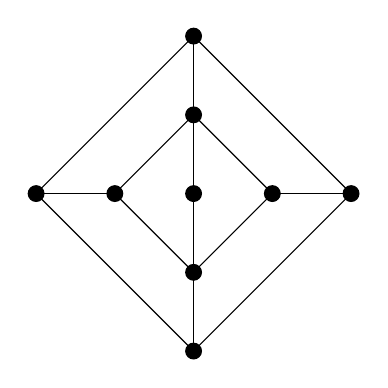
\begin{tikzpicture}
                \draw[fill] (-2,0) circle [radius=0.1];
                \draw[fill] (-1,0) circle [radius=0.1];
                \draw[fill] (0,0) circle [radius=0.1];
                \draw[fill] (1,0) circle [radius=0.1];
                \draw[fill] (2,0) circle [radius=0.1];
                \draw[fill] (0,-2) circle [radius=0.1];
                \draw[fill] (0,-1) circle [radius=0.1];
                \draw[fill] (0,1) circle [radius=0.1];
                \draw[fill] (0,2) circle [radius=0.1];
                \draw (-2,0)--(-1,0);
                \draw (1,0)--(2,0);
                \draw (-2,0)--(0,-2);
                \draw (-2,0)--(0,2);
                \draw (0,-2)--(2,0);
                \draw (0,2)--(2,0);
                \draw (0,-2)--(0,2);
                \draw (-1,0)--(0,-1);
                \draw (-1,0)--(0,1);
                \draw (0,-1)--(1,0);
                \draw (0,1)--(1,0);
            \end{tikzpicture}
            \end{center}
}}}\bigskip\par

Every edge in this graph connects a red and a blue node. Since a Hamiltonian cycle is a subgraph, it would also have that property, so it would visit the same number of red and blue vertices. However, to be a Hamiltonian cycle, it must visit each of the 4 blue vertices and the 5 red vertices exactly once. That's a contradiction, so the graph is not Hamiltonian.
\begin{center}
    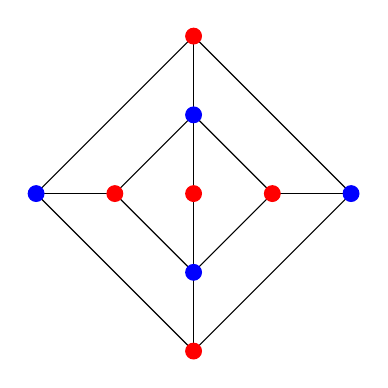
\begin{tikzpicture}
        \draw (-2,0)--(-1,0);
        \draw (1,0)--(2,0);
        \draw (-2,0)--(0,-2);
        \draw (-2,0)--(0,2);
        \draw (0,-2)--(2,0);
        \draw (0,2)--(2,0);
        \draw (0,-2)--(0,2);
        \draw (-1,0)--(0,-1);
        \draw (-1,0)--(0,1);
        \draw (0,-1)--(1,0);
        \draw (0,1)--(1,0);
        \draw[fill, blue] (-2,0) circle [radius=0.1];
        \draw[fill, red ] (-1,0) circle [radius=0.1];
        \draw[fill, red ] (0,0) circle [radius=0.1];
        \draw[fill, red ] (1,0) circle [radius=0.1];
        \draw[fill, blue] (2,0) circle [radius=0.1];
        \draw[fill, red ] (0,-2) circle [radius=0.1];
        \draw[fill, blue] (0,-1) circle [radius=0.1];
        \draw[fill, blue] (0,1) circle [radius=0.1];
        \draw[fill, red ] (0,2) circle [radius=0.1];
    \end{tikzpicture}
\end{center}

\section{}
\noindent\fbox{\fbox{\parbox{6.5in}{
            Prove that if an edge $e$ appears an odd number of times in a closed walk $W$, then $W$ contains the edges of a cycle through $e$. \textit{Hint: Use induction on the length of $W$}.
}}}\bigskip\par

\section{}
\noindent\fbox{\fbox{\parbox{6.5in}{
    \textbf{Section 4.4, Exercise 10}
    \begin{center}
        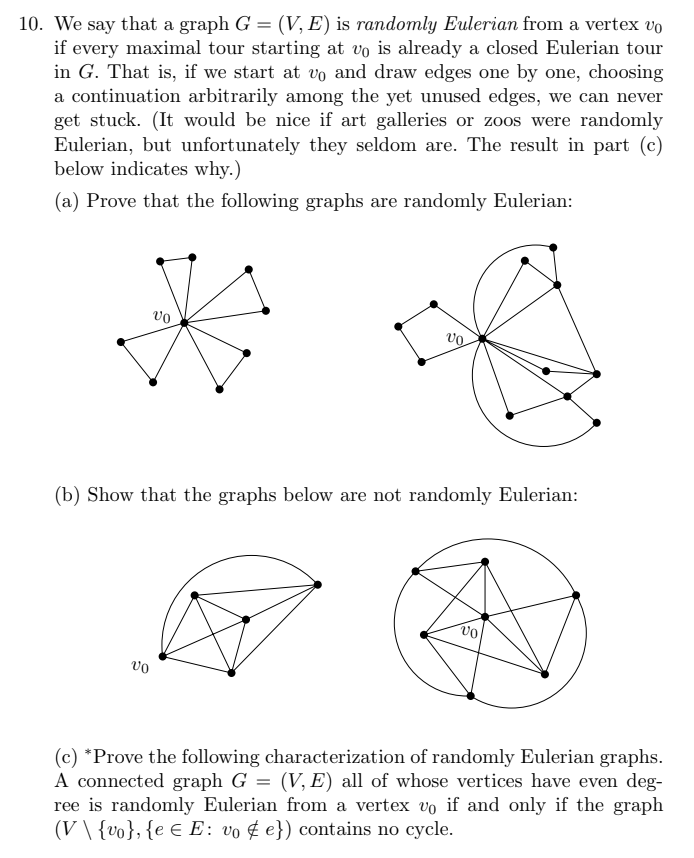
\includegraphics[width=\textwidth]{Screenshot from 2024-01-29 07-28-21.png}
    \end{center}
}}}\bigskip\par

\end{document}
